\apendice{Especificación de diseño}

\section{Introducción}
Una vez realizado el estudio y especificación de los requisitos de la aplicación web, se debe realizar el diseño de la misma. En este anexo se pretende aportar información sobre el diseño de los datos que utiliza la aplicación junto al diseño procedimental y arquitectónico del proyecto.

\section{Diseño de datos}
Gracias a la especificación de requisitos y casos de uso, se puede obtener una visión global de la aplicación que permite deducir las entidades, acompañadas de sus datos, necesarias para poder cumplir con lo requerido.

En primer lugar, podemos obtener la visión global de las entidades relacionadas mediante el diagrama general de Entidad-Relación de la figura~\ref{DiagramaGeneralE-R}.

El diagrama obtenido tiene un gran tamaño y, para mejorar la visualización y comprensión del mismo, se ha decidido dividir en vistas donde se incluyan los datos de cada una de las entidades.

La primera vista hace referencia al apartado de mantenimiento académico y se puede ver en la figura~\ref{er_cu1}, la segunda al mantenimiento de profesorado~\ref{er_cu2} y la última a la asignación docente~\ref{er_cu3}.


\figuraApaisadaSinMarco{}{../img/Anexos/Diagrama E-R.pdf}{Diagrama general entidad-relación}{DiagramaGeneralE-R}{}

Del diagrama entidad-relación se puede obtener el diagrama relacional de la figura~\ref{DiagramaRelacional} en el que se pueden ver la tablas que contendrá la base de datos de la aplicación web.

En este diagrama se pueden ver las tablas de la base de datos juntos los distintos campos que tendrá cada una.
Como se puede ver en la figura~\ref{DiagramaRelacional}, las tablas centro, titulación y asignatura tienen un campo llamado código. 
Este código campo podría haber sido utilizado como clave primaria, pero al ser un campo que introduce el usuario, se decidió mantener una clave primaria auto-incremental con la que se hacen las relaciones de las tablas, y además, añadir ese campo para que se puedan hacer búsquedas o filtrar por el mismo sin que su uso pueda afectar a la consistencia del sistema.

Otro aspecto relevante es que en las relaciones que dan lugar a la creación de una tabla intermedia se siguió el mismo patrón que antes. 
Aunque la teoría diga que las claves de las tablas que se relacionan pasan a ser claves primarias de la nueva tabla que se genera, se decidió tener una única clave primaria auto-incremental y tener las claves de las tablas relacionadas como claves foráneas.
De esta manera, las búsquedas en la base de datos estarán más optimizadas al buscar como clave primaria un único campo y no la composición de varios.
Además, se evita cualquier tipo de error de clave primaria al ser la propia base de datos la que asigna esta y no el código creado.

\figuraApaisadaSinMarco{.93}{../img/Anexos/Diagrama relacional.pdf}{Diagrama relacional}{DiagramaRelacional}{}

\subsection{Diccionario de datos}
A continuación se va a especificar, para cada tabla de la base de datos, el diccionario de datos correspondiente.
De esta forma se pretende facilitar la comprensión de los datos almacenados en la base de datos.

La tabla \texttt{centro} almacena los diferentes centros de la universidad. 
Se puede ver su información en la tabla~\ref{tab:diccionario_centro}.
\begin{table}
\centering
  \begin{tabular}{l p{.2\textwidth} p{.5\textwidth}}
    \toprule
    \textbf{Campo} & \textbf{Tipo} & \textbf{Descripción}\\
    \midrule
    \textbf{\underline{id}} & Entero \underline{PK} & Identificador. Clave primaria creada de forma autoincremental. \\ \addlinespace
    codigo & Entero & Código interno del centro de la universidad. Sólo tiene carácter informativo. \\ \addlinespace 
    abreviatura & Texto & Abreviatura del centro. \\ \addlinespace
    email & Texto & Email administrativo del centro. \\
    \bottomrule
  \end{tabular}
  \caption{Diccionario de datos. Tabla Centro}
  \label{tab:diccionario_centro}
\end{table}

La tabla \texttt{titulación} almacena las titulaciones que son creadas y que pertenecen a un centro.
Se puede ver su información en la tabla~\ref{tab:diccionario_titulacion}.
\begin{table}
  \centering 
  \begin{tabular}{l p{.2\textwidth} p{.5\textwidth}}
    \toprule
    \textbf{Campo} & \textbf{Tipo} & \textbf{Descripción}\\
    \midrule
    \textbf{\underline{id}} & Entero \underline{PK} & Identificador de la titulación. Clave primaria creada de forma autoincremental. \\ \addlinespace
    codigo & Entero & Código interno de la titulación. \\ \addlinespace
    nombre & Texto & Nombre de la titulación. \\ \addlinespace
    abreviatura & Texto & Abreviatura de la titulación. \\ \addlinespace
    url & Texto & Dirección web de la titulación. \\ \addlinespace
    id\_centro & Entero FK(Centro) & Identificador del centro asociado a la titulación. \\
    \bottomrule
  \end{tabular}
  \caption{Diccionario de datos. Tabla Titulación}
  \label{tab:diccionario_titulacion}
\end{table}

La tabla \texttt{asignatura} almacena información sobre las asignaturas, cada asignatura pertenece a una titulación. Se puede ver su información en la tabla~\ref{tab:diccionario_asignatura}.

\begin{table}
  \centering 
  \begin{tabular}{l p{.2\textwidth} p{.5\textwidth}}
    \toprule
    \textbf{Campo} & \textbf{Tipo} & \textbf{Descripción}\\
    \midrule
    \textbf{\underline{id}} & Entero \underline{PK} & Identificador de la asignatura. Clave primaria creada de forma autoincremental. \\ \addlinespace
    codigo & Entero & Código interno de la asignatura. \\ \addlinespace
    nombre & Texto & Nombre de la asignatura. \\ \addlinespace
    tipo & Texto & Tipo de la asignatura. \\ \addlinespace
    creditos\_teoria & Entero & Créditos de teoría de la asignatura. \\ \addlinespace
    creditos\_practica & Entero & Créditos de práctica de la asignatura. \\ \addlinespace
    curso & Texto & Curso al que pertenece la asignatura. \\ \addlinespace
    semestre & Texto & Semestre en el que se imparte la asignatura. \\ \addlinespace
    id\_titulacion & Entero FK(Titulación) & Identificador de la titulación a la que pertenece la asignatura. \\
    \bottomrule
  \end{tabular}
  \caption{Diccionario de datos. Tabla Asignatura}
  \label{tab:diccionario_asignatura}
\end{table}

La tabla \texttt{abreviatura} almacena las abreviaturas de las asignaturas. 
De esta forma se permite que una asignatura pueda tener varias abreviaturas.
Se puede ver su información en la tabla~\ref{tab:diccionario_abreviatura}.

\begin{table}
  \centering 
  \begin{tabular}{l p{.2\textwidth} p{.5\textwidth}}
    \toprule
    \textbf{Campo} & \textbf{Tipo} & \textbf{Descripción}\\
    \midrule
    \textbf{\underline{id}} & Entero \underline{PK} & Identificador de la abreviatura. Clave primaria creada de forma autoincremental. \\ \addlinespace
    abreviatura & Texto & Abreviatura de la asignatura. \\ \addlinespace
    id\_asignatura & Entero FK(Asignatura) & Identificador de la asignatura asociada a la abreviatura. \\
    \bottomrule
  \end{tabular}
  \caption{Diccionario de datos. Tabla Abreviatura}
  \label{tab:diccionario_abreviatura}
\end{table}

La tabla \texttt{curso} almacena información sobre los cursos. Se puede ver su información en la tabla~\ref{tab:diccionario_curso}.

\begin{table}
  \centering 
  \begin{tabular}{l p{.2\textwidth} p{.5\textwidth}}
    \toprule
    \textbf{Campo} & \textbf{Tipo} & \textbf{Descripción}\\
    \midrule
    \textbf{\underline{id}} & Entero \underline{PK} & Identificador del curso. Clave primaria creada de forma autoincremental. \\ \addlinespace
    ano\_inicio & Texto & Año de inicio del curso. \\ \addlinespace
    \bottomrule
  \end{tabular}
  \caption{Diccionario de datos. Tabla Curso}
  \label{tab:diccionario_curso}
\end{table}

La tabla \texttt{curso\_asignatura} almacena la relación entre cursos y asignaturas. 
Se puede ver su información en la tabla~\ref{tab:diccionario_curso_asignatura}.

\begin{table}
  \centering
  \begin{tabular}{l p{.2\textwidth} p{.25\textwidth}}
    \toprule
    \textbf{Campo} & \textbf{Tipo} & \textbf{Descripción}\\
    \midrule
    \textbf{\underline{id}} & Entero \underline{PK} & Identificador de la relación curso-asignatura. Clave primaria creada de forma autoincremental. \\ \addlinespace
    id\_asignatura & Entero FK(Asignatura) & Identificador de la asignatura relacionada. \\ \addlinespace
    id\_curso & Entero FK(Curso) & Identificador del curso relacionado. \\ \addlinespace
    modalidad & Texto & Modalidad de la relación curso-asignatura. \\ \addlinespace
    num\_alumnos\_previstos & Entero & Número de alumnos previstos para la relación curso-asignatura. \\ \addlinespace
    num\_grupos\_teoricos\_previstos & Entero & Número de grupos teóricos previstos para la relación curso-asignatura. \\ \addlinespace
    num\_grupos\_practicos\_previstos & Entero & Número de grupos prácticos previstos para la relación curso-asignatura. \\
    \bottomrule
  \end{tabular}
  \caption{Diccionario de datos. Tabla Curso-Asignatura}
  \label{tab:diccionario_curso_asignatura}
\end{table}

La tabla \texttt{grupo} almacena información sobre los grupos de asignaturas. 
Se puede ver su información en la tabla~\ref{tab:diccionario_grupo}.

\begin{table}
  \centering 
  \begin{tabular}{l p{.2\textwidth} p{.4\textwidth}}
    \toprule
    \textbf{Campo} & \textbf{Tipo} & \textbf{Descripción}\\
    \midrule
    \textbf{\underline{id}} & Entero \underline{PK} & Identificador del grupo. Clave primaria creada de forma autoincremental. \\ \addlinespace
    nombre & Texto & Nombre del grupo. \\ \addlinespace
    tipo & Texto & Tipo de grupo. \\ \addlinespace
    id\_curso\_asignatura & Entero FK(Curso-Asignatura) & Identificador de la relación curso-asignatura asociada al grupo. \\
    \bottomrule
  \end{tabular}
  \caption{Diccionario de datos. Tabla Grupo}
  \label{tab:diccionario_grupo}
\end{table}

La tabla \texttt{docente} almacena información sobre los docentes. Se puede ver su información en la tabla~\ref{tab:diccionario_docente}.

\begin{table}
  \centering 
  \begin{tabular}{l p{.2\textwidth} p{.5\textwidth}}
    \toprule
    \textbf{Campo} & \textbf{Tipo} & \textbf{Descripción}\\
    \midrule
    \textbf{\underline{id}} & Entero \underline{PK} & Identificador del docente. Clave primaria generada de forma autoincremental. \\ \addlinespace
    nombre & Texto & Nombre del docente. \\ \addlinespace
    apellidos & Texto & Apellidos del docente. \\ \addlinespace
    email & Texto & Email del docente \\ \addlinespace
    reducciones & Entero & Número de horas de reducciones del docente. \\ \addlinespace
    read\_flag & \textit{Boolean} & Permisos de lectura. \\ \addlinespace
    modification\_flag & \textit{Boolean} & Permisos de modificación. \\
    \bottomrule
  \end{tabular}
  \caption{Diccionario de datos. Tabla Docente}
  \label{tab:diccionario_docente}
\end{table}

La tabla \texttt{departamento} almacena información sobre los departamentos de la universidad. 
Se puede ver su información en la tabla~\ref{tab:diccionario_departamento}.

\begin{table}
  \centering 
  \begin{tabular}{l p{.2\textwidth} p{.5\textwidth}}
    \toprule
    \textbf{Campo} & \textbf{Tipo} & \textbf{Descripción}\\
    \midrule
    \textbf{\underline{id}} & Entero \underline{PK} & Identificador del departamento. Clave primaria generada de forma autoincremental. \\ \addlinespace
    nombre & Texto & Nombre del departamento. \\ \addlinespace
    abreviatura & Texto & Abreviatura del departamento. \\
    \bottomrule
  \end{tabular}
  \caption{Diccionario de datos. Tabla Departamento}
  \label{tab:diccionario_departamento}
\end{table}

La tabla \texttt{área} almacena información sobre las áreas de un departamento. 
Se puede ver su información en la tabla~\ref{tab:diccionario_area}.

\begin{table}
  \centering 
  \begin{tabular}{l p{.3\textwidth} p{.4\textwidth}}
    \toprule
    \textbf{Campo} & \textbf{Tipo} & \textbf{Descripción}\\
    \midrule
    \textbf{\underline{id}} & Entero \underline{PK} & Identificador del área. Clave primaria creada de forma autoincremental. \\ \addlinespace
    nombre & Texto & Nombre del área. \\ \addlinespace
    abreviatura & Texto & Abreviatura del área. \\ \addlinespace
    id\_departamento & Entero FK(Departamento) & Identificador del departamento al que pertenece el área. \\
    \bottomrule
  \end{tabular}
  \caption{Diccionario de datos. Tabla Área}
  \label{tab:diccionario_area}
\end{table}

La tabla \texttt{contrato} almacena información sobre los tipos de contratos. 
Se puede ver su información en la tabla~\ref{tab:diccionario_tipo_contrato}.

\begin{table}
  \centering 
  \begin{tabular}{l p{.2\textwidth} p{.5\textwidth}}
    \toprule
    \textbf{Campo} & \textbf{Tipo} & \textbf{Descripción}\\
    \midrule
    \textbf{\underline{id}} & Entero \underline{PK} & Identificador del tipo de contrato. Clave primaria generada de forma autoincremental. \\ \addlinespace
    nombre & Texto & Nombre del tipo de contrato. \\ \addlinespace
    abreviatura & Texto & Abreviatura del tipo de contrato. \\ \addlinespace
    capacidad\_anual & Entero & Capacidad anual en horas del tipo de contrato. \\
    \bottomrule
  \end{tabular}
  \caption{Diccionario de datos. Tabla Tipo Contrato}
  \label{tab:diccionario_tipo_contrato}
\end{table}

La tabla \texttt{plaza} almacena información sobre las plazas de contratación. 
Se puede ver su información en la tabla~\ref{tab:diccionario_plaza}.

\begin{table}
  \centering 
  \begin{tabular}{l p{.2\textwidth} p{.35\textwidth}}
    \toprule
    \textbf{Campo} & \textbf{Tipo} & \textbf{Descripción}\\
    \midrule
    \textbf{\underline{id}} & Entero \underline{PK} & Identificador de la plaza. Clave primaria generada de forma autoincremental \\ \addlinespace
    nombre & Texto & Nombre de la plaza \\ \addlinespace
    rpt & Texto & RPT de la plaza \\ \addlinespace
    num\_concursos\_contratacion & Entero & Número de concursos de contratación de la plaza \\ \addlinespace
    fecha\_incorporacion & Fecha & Fecha de incorporación a la plaza. \\ \addlinespace
    fecha\_cese & Fecha & Fecha de cese de la plaza. \\ \addlinespace
    id\_docente & Entero & Identificador del docente asignado a la plaza. \\ \addlinespace
    id\_area & Entero & Identificador del área asociada a la plaza. \\ \addlinespace
    id\_contrato & Entero & Identificador del tipo de contrato asociado a la plaza. \\ \addlinespace
    observaciones & Texto & Observaciones de la plaza. \\ \addlinespace
    \bottomrule
  \end{tabular}
  \caption{Diccionario de datos. Tabla Plaza}
  \label{tab:diccionario_plaza}
\end{table}

La tabla \texttt{plaza-grupo} almacena información sobre la asignación de horas de plazas a grupos. 
Se puede ver su información en la tabla~\ref{tab:diccionario_plaza_grupo}.

\begin{table}
  \centering 
  \begin{tabular}{l p{.2\textwidth} p{.5\textwidth}}
    \toprule
    \textbf{Campo} & \textbf{Tipo} & \textbf{Descripción}\\
    \midrule
    \textbf{\underline{id}} & Entero \underline{PK} & Identificador de la asignación. Clave primaria generada de forma autoincremental. \\ \addlinespace
    horas & Entero & Horas de la plaza asignadas al grupo. \\ \addlinespace
    id\_grupo & Entero & Identificador del grupo. \\ \addlinespace
    id\_plaza & Entero & Identificador de la plaza. \\ 
    \bottomrule
  \end{tabular}
  \caption{Diccionario de datos. Tabla Plaza-Grupo}
  \label{tab:diccionario_plaza_grupo}
\end{table}

Existen otras dos tablas llamadas \texttt{alemic\_version} y \texttt{sessions} que son creadas por algunas de las bibliotecas que se utilizan en la aplicación. 
La primera guarda un registro de las migraciones de la base de datos y la segunda almacena la sesión de los usuarios.

\section{Diseño procedimental}
El diseño procedimental es una fase fundamental en el desarrollo de proyectos informáticos, donde se establecen los pasos necesarios para realizar una actividad dentro de la aplicación.

\begin{itemize}
\item \textbf{Creación de centro}

El diagrama~\ref{DS-crearCentro} muestra los pasos necesarios para crear un nuevo centro en la aplicación web.

Se parte de que el usuario está en la ventana de centros.
Desde ahí el usuario debe pulsar en <<Nuevo>>, lo que provocará la redirección a la ventana que contiene el formulario de creación.
El usuario debe rellenar el formulario y pulsar sobre <<Añadir>>.

Al hacer esto los datos se mandan al servidor.
Si todo está correcto el nuevo centro se almacena en la base de datos, mientras que si hay algún error en los datos introducidos, se recarga la página del formulario indicando los errores de cada campo.

El método \texttt{save} se encarga de comprobar si el objeto centro tiene identificador, ya que si no tiene, se trata de un objeto no almacenado en la base de datos y debe llamar al método \texttt{add} para guardarlo, mientras que si ya tiene id, quiere decir que se trata de una modificación y tan sólo debe hacer el \textit{commit} para guardar los datos modificados.

Una vez se ha guardado el nuevo centro, la aplicación redirecciona al usuario a la página de centros.

El diagrama~\ref{DS-crearCentro} se va a utilizar como ejemplo de creación para las tablas de <<Titulación>>, <<Asignatura>>, <<Docente>>, <<Plaza>>, <<Contrato>>, <<Área>> y <<Departamento>>.
Esto es debido a que la creación en estas tablas es igual y sólo cambia el nombre de los modelos, controladores y rutas, pero el funcionamiento es el mismo.

\begin{figure}
	\centering
	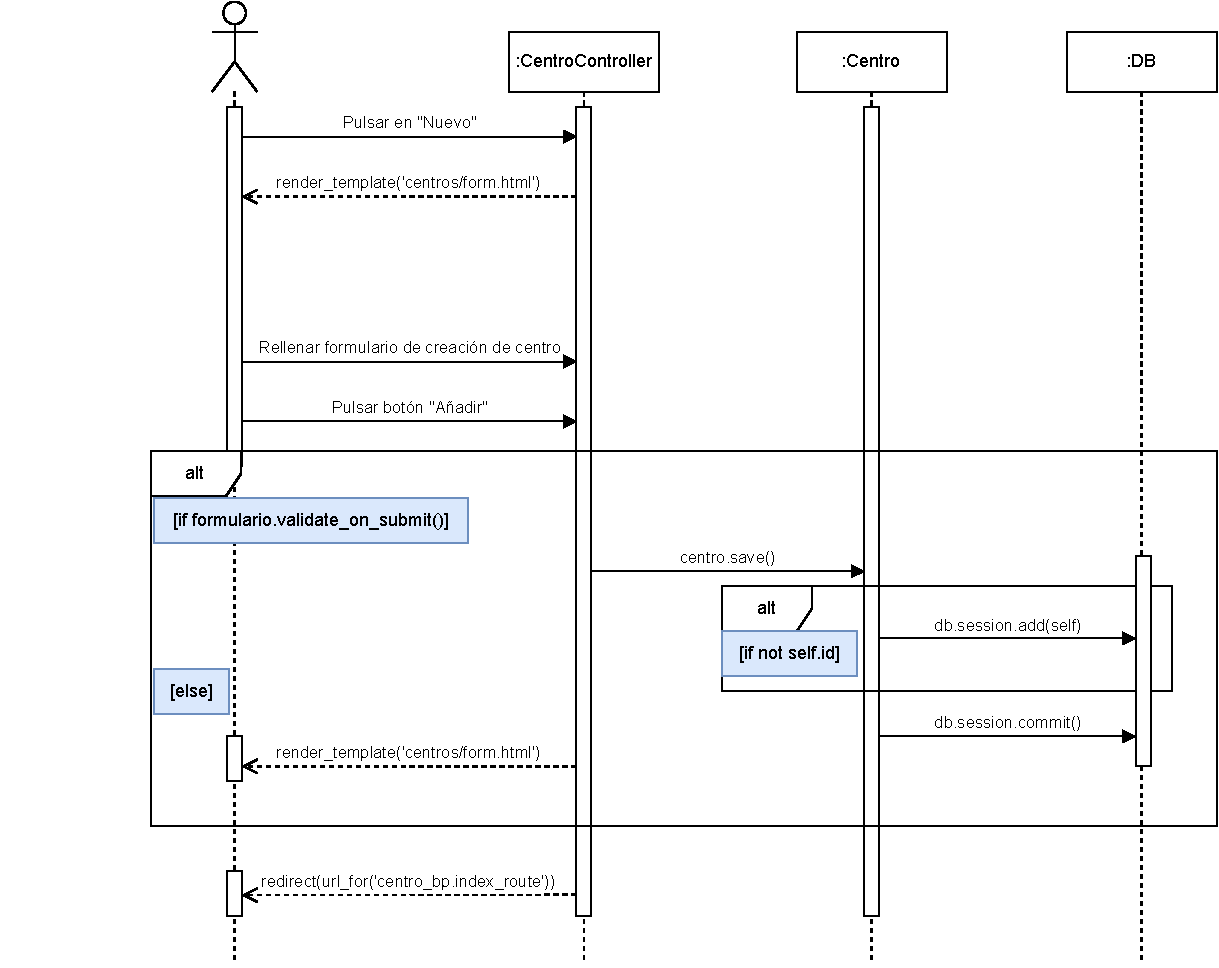
\includegraphics[width=\textwidth]{../img/Anexos/Diagramas secuencia/DS - crear centro.pdf}
	\caption{Diagrama de secuencia referente a la creación de centros.}\label{DS-crearCentro}
\end{figure}

\item \textbf{Modificación de centro}

En el diagrama~\ref{DS-modificarCentro} se muestra el proceso seguido para modificar un centro.
Se parte de la base de que el centro ya se encuentra creado.
Al igual que en el caso anterior, este diagrama sirve de ejemplo para la modificación de <<Titulación>>, <<Asignatura>>, <<Docente>>, <<Plaza>>, <<Contrato>>, <<Área>> y <<Departamento>>.

Suponiendo que el usuario se encuentra en la ventana de centros y que ahí por lo menos un centro creado, pulsa en el icono de lápiz de uno de los centros de la lista.

Al realizar esta acción se abre un formulario con los datos del centro seleccionado.
Desde aquí el usuario puede cambiar los campos que quiera.
Una vez realizados los cambios debe pulsar sobre <<Modificar>>.

Una vez modificados los campos y pulsada la opción indicada anteriormente, el servidor recogerá los datos. 
Si todo está bien, las modificaciones se almacenarán en la base de datos y el usuario será redirigido a la ventana principal de los centros.
En caso contrario, se recargará la página del formulario indicando los campos que tienen errores y qué errores son.

\begin{figure}
	\centering
	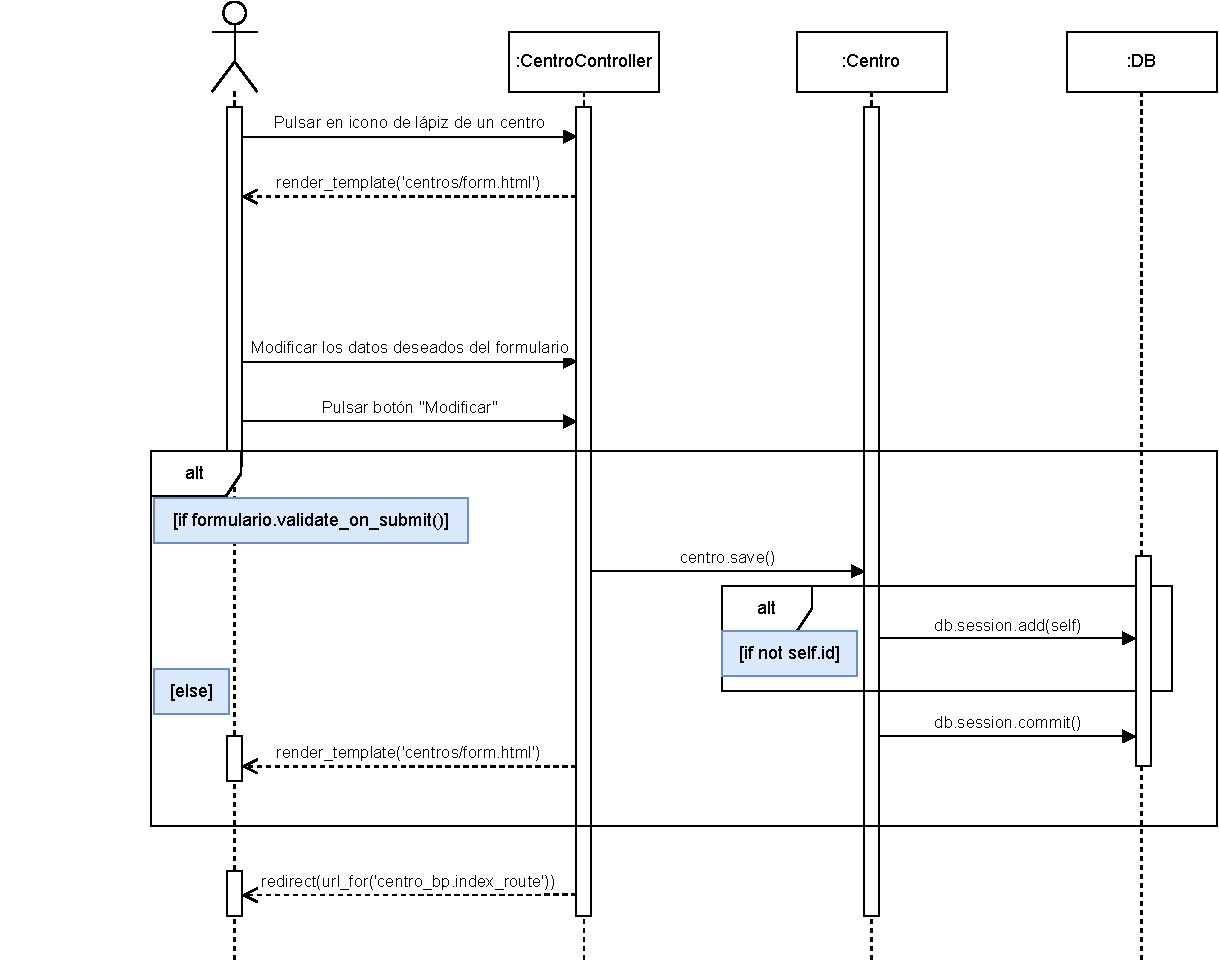
\includegraphics[width=\textwidth]{../img/Anexos/Diagramas secuencia/DS - modificar centro.pdf}
	\caption{Diagrama de secuencia referente a la modificación de centros.}\label{DS-modificarCentro}
\end{figure}

\item \textbf{Eliminación de centro}

El diagrama~\ref{DS-eliminarCentro} muestra al secuencia de pasos que se siguen para eliminar un centro de la aplicación.

Partiendo de la base de que existe al menos un centro creado y que el usuario se encuentra en la ventana de centros, el usuario pulsar sobre el icono de una papelera de un centro de la tabla.
Al realizar esta acción aparece una ventana de confirmación para afirmar que se quiere eliminar el centro. 
Al pulsar en aceptar se manda al servidor la petición de eliminación.

En el servidor se comprobará si el centro existe. 
Si no existe se devolverá un error 404 mientras que si existe se comprobará si el centro tiene titulaciones que dependan de él.
En caso afirmativo se redireccionará al usuario a la ventana principal de centros indicando que no se puede eliminar el centro porque tiene titulaciones asociadas.
En caso de que el centro no tenga titulaciones asociadas, se eliminará de la base de datos y se redireccionará al usuario a la vista principal de centros indicando en un mensaje que el centro se ha eliminado correctamente.

\begin{figure}
	\centering
	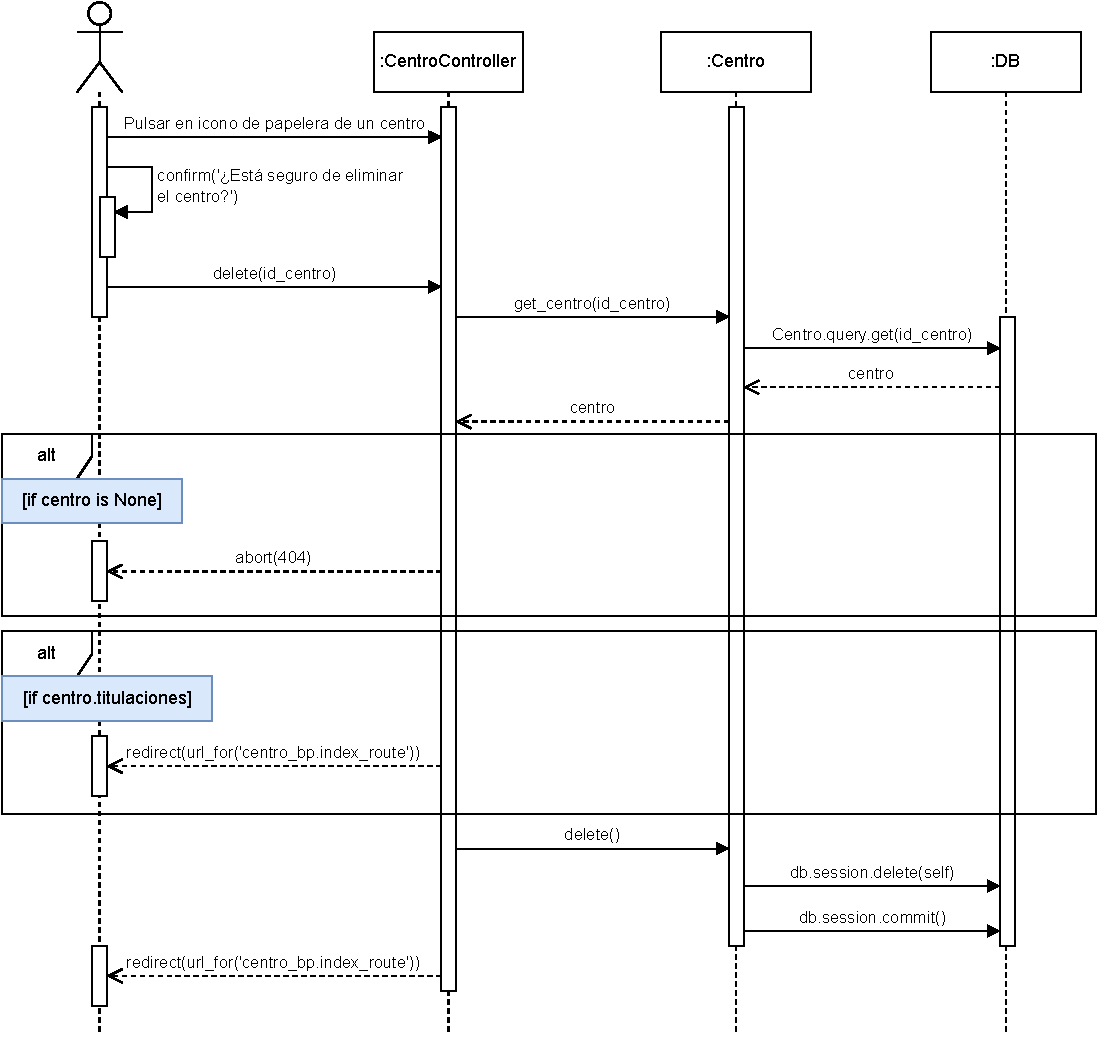
\includegraphics[width=\textwidth]{../img/Anexos/Diagramas secuencia/DS - eliminar centro.pdf}
	\caption{Diagrama de secuencia de la eliminación de centros.}\label{DS-eliminarCentro}
\end{figure}

\item \textbf{Asignar plaza a docente}

En el diagrama~\ref{DS-asignarPlaza} se puede ver el conjunto de pasos seguidos para asignar una plaza a un docente.
Para este caso se supone que se tiene una plaza y un docente creados previamente.

El cliente pulsa en el icono del lápiz de una de las plazas.
Esto abre el formulario de edición de la plaza desde donde puede seleccionar el docente a través del campo de búsqueda de docentes escribiendo el nombre del mismo.
Con el docente seleccionado se pulsa en <<Modificar>>.

Si todos los campos del formulario son correctos, se comprueba si el docente tiene alguna plaza sin fecha de cese, en ese caso no se puede vincular con esta plaza y se mostrará un mensaje informando del error. 
En caso contrario, la plaza se asigna.

Finalmente, los cambios se guardan en la base de datos y se redirecciona al usuario a la vista de plazas donde se muestran los mensajes correspondientes a la correcta modificación de la plaza y, si no ha sido posible asignar la plaza por culpa de poseer alguna plaza sin fecha de cese, también se muestra en un mensaje de error.
En caso de no haber pasado la validación del formulario, se redirecciona a la ventana del formulario mostrando los errores detectados.

\begin{figure}
	\centering
	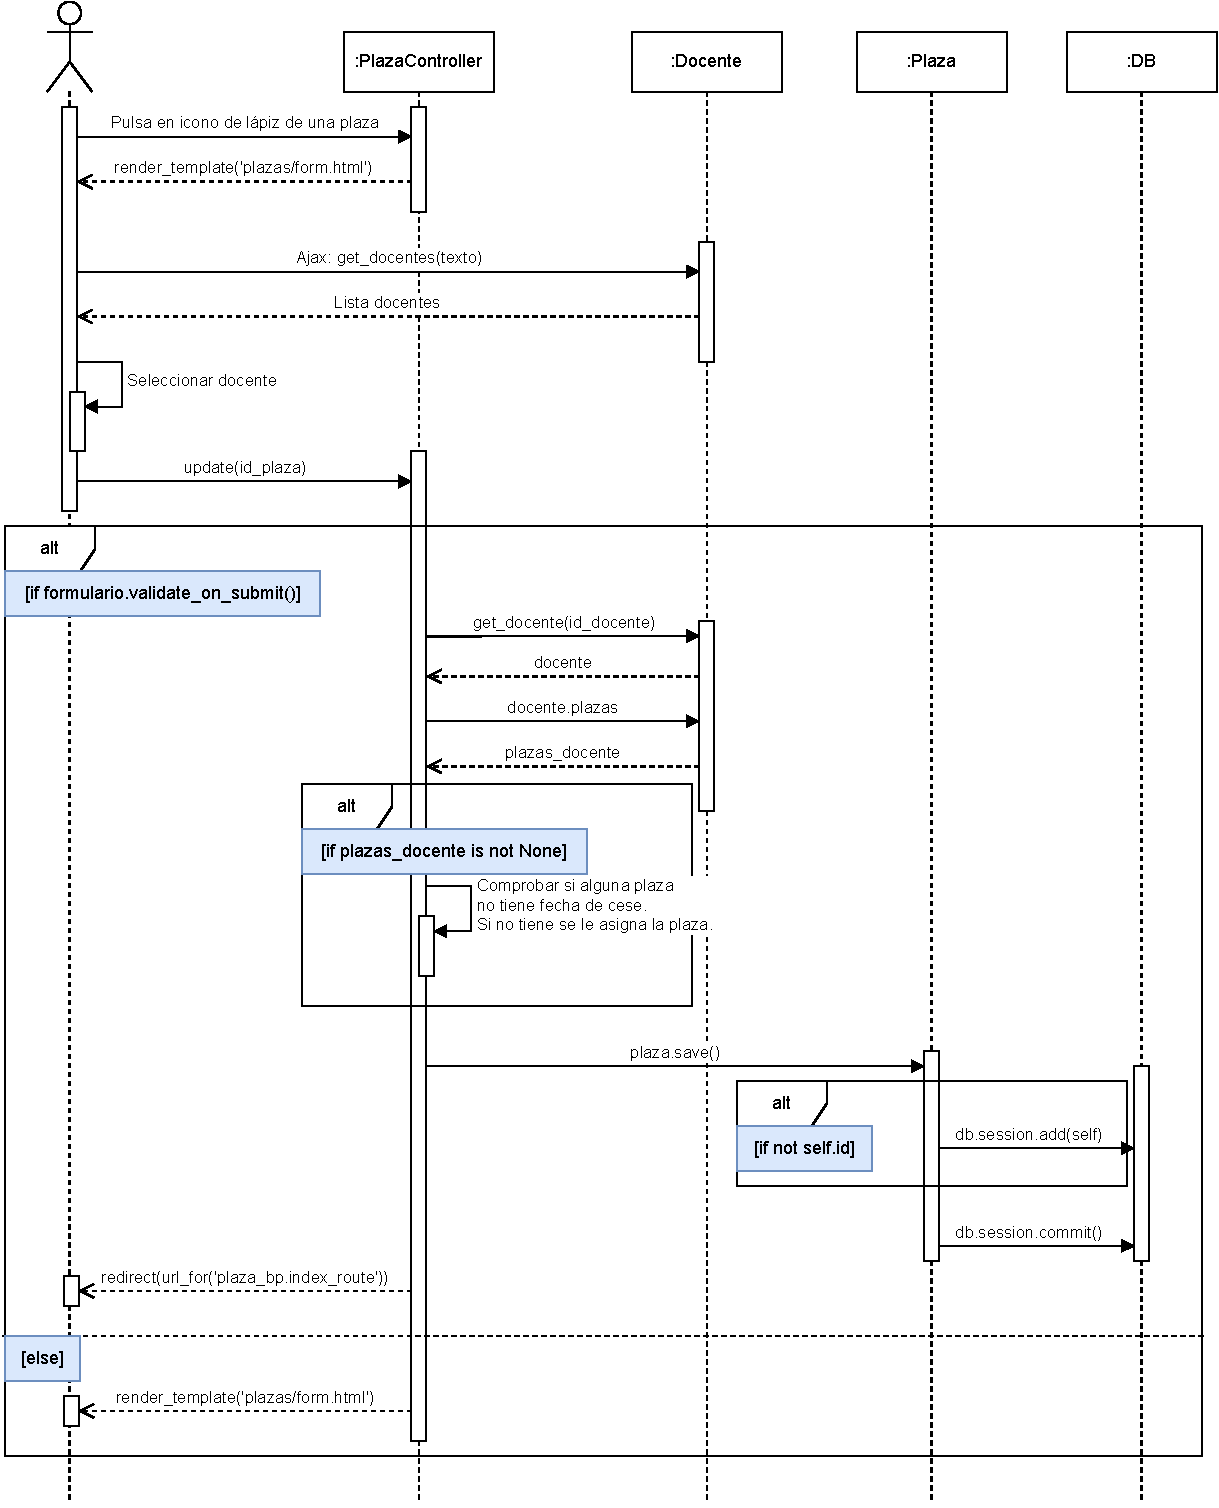
\includegraphics[width=\textwidth]{../img/Anexos/Diagramas secuencia/DS - asignar plaza.pdf}
	\caption{Diagrama de secuencia de la asignación de una plaza a un docente.}\label{DS-asignarPlaza}
\end{figure}

\item \textbf{Creación de curso académico}

El diagrama~\ref{DS-crearCurso} contiene los pasos necesarios para crear un nuevo curso académico.

El usuario parte de la ventana de cursos donde debe pulsar sobre <<Nuevo>>. Esto abre una ventana donde se indica el año de inicio del nuevo curso a crear y se pulsa sobre <<Añadir>>.

Con el paso anterior realizado, el usuario se encuentra en la ventana donde puede seleccionar el número de alumnos de cada modalidad y las asignaturas que quiere incluir al curso. Después de realizar la selección deseada pulsa sobre <<Añadir>>. Esto hará que se cree la vinculación entre el curso y aquellas asignaturas que no están ya vinculadas. Además, se crea un grupo de tipo presencial y otro de tipo práctico por cada asignatura.

En caso de producirse algún error con el formulario de introducción de año, como por ejemplo añadir un año de un curso existente, se devolverá al usuario a la ventana del formulario indicando el error. Lo mismo ocurre en el formulario de selección de asignaturas, si el formulario no se valida correctamente, se le mostrará el error al usuario en el propio formulario.

Si al final todo ha ido bien, el usuario será redirigido a la ventana principal de cursos donde podrá ver el curso creado y un mensaje indicando la correcta creación y asignación de asignaturas realizada.


\begin{figure}
	\centering
	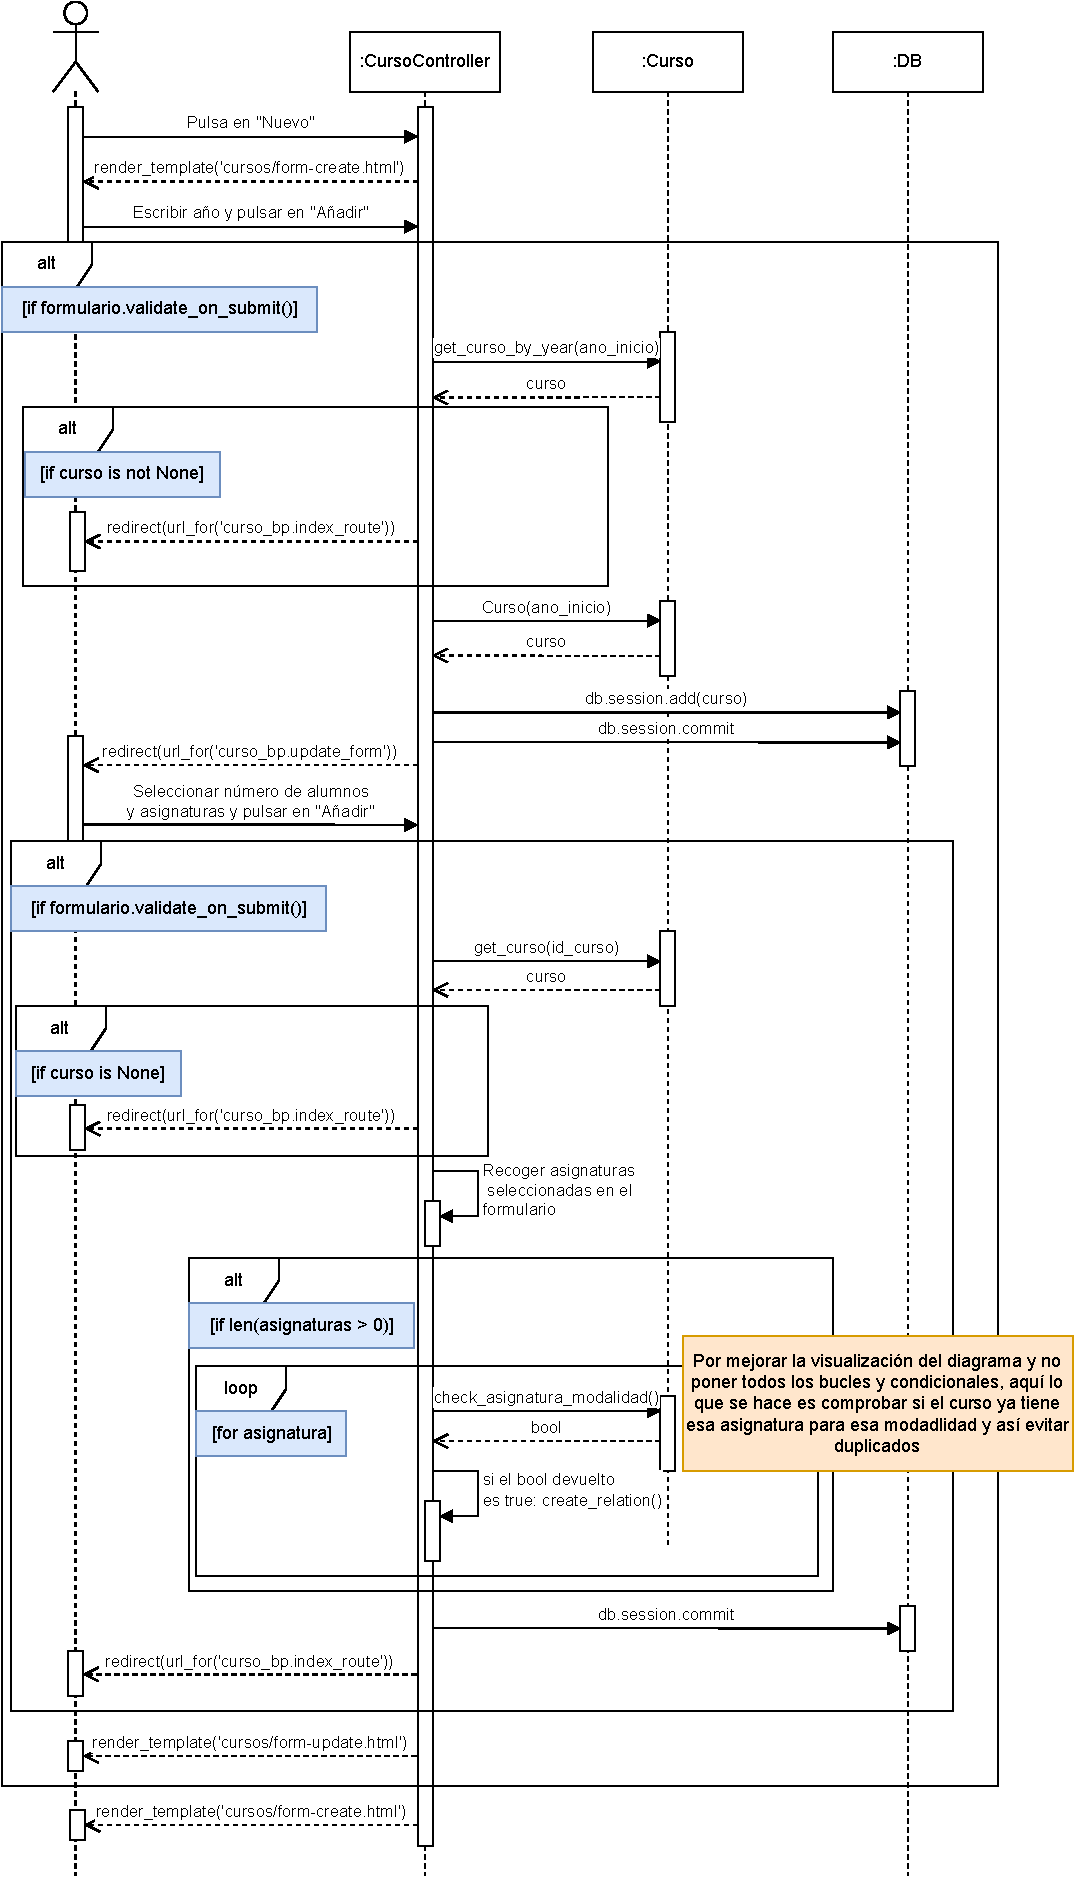
\includegraphics[width=.9\textwidth]{../img/Anexos/Diagramas secuencia/DS - crear curso.pdf}
	\caption{Diagrama de secuencia de la creación de un curso académico.}\label{DS-crearCurso}
\end{figure}


\item \textbf{Creación de grupo}

En el diagrama~\ref{DS-crearGrupo} se muestra el proceso seguido para crear un nuevo grupo en una asignatura vinculada a un curso académico. Se parte de la base de que existe un curso con al menos una asignatura y que el usuario se encuentra en la ventana de grupos donde aparece un listado de las asignaturas del curso académico.

El usuario comienza el proceso pulsando sobre el icono de dos personas de una asignatura del listado. De esta manera será redirigido a la vista de los grupos de la asignatura. Acto seguido pulsa sobre el botón <<Añadir grupo>>, lo que abre una ventana modal donde podrá seleccionar entre las modalidades teórico o presencial para el nuevo grupo a crear. Una vez seleccionada esta opción, pulsa sobre el botón <<Añadir>> y la ventana modal se cerrará. Además, aparecerá un mensaje informando de la creación y se podrá ver el grupo en la lista.

\begin{figure}
	\centering
	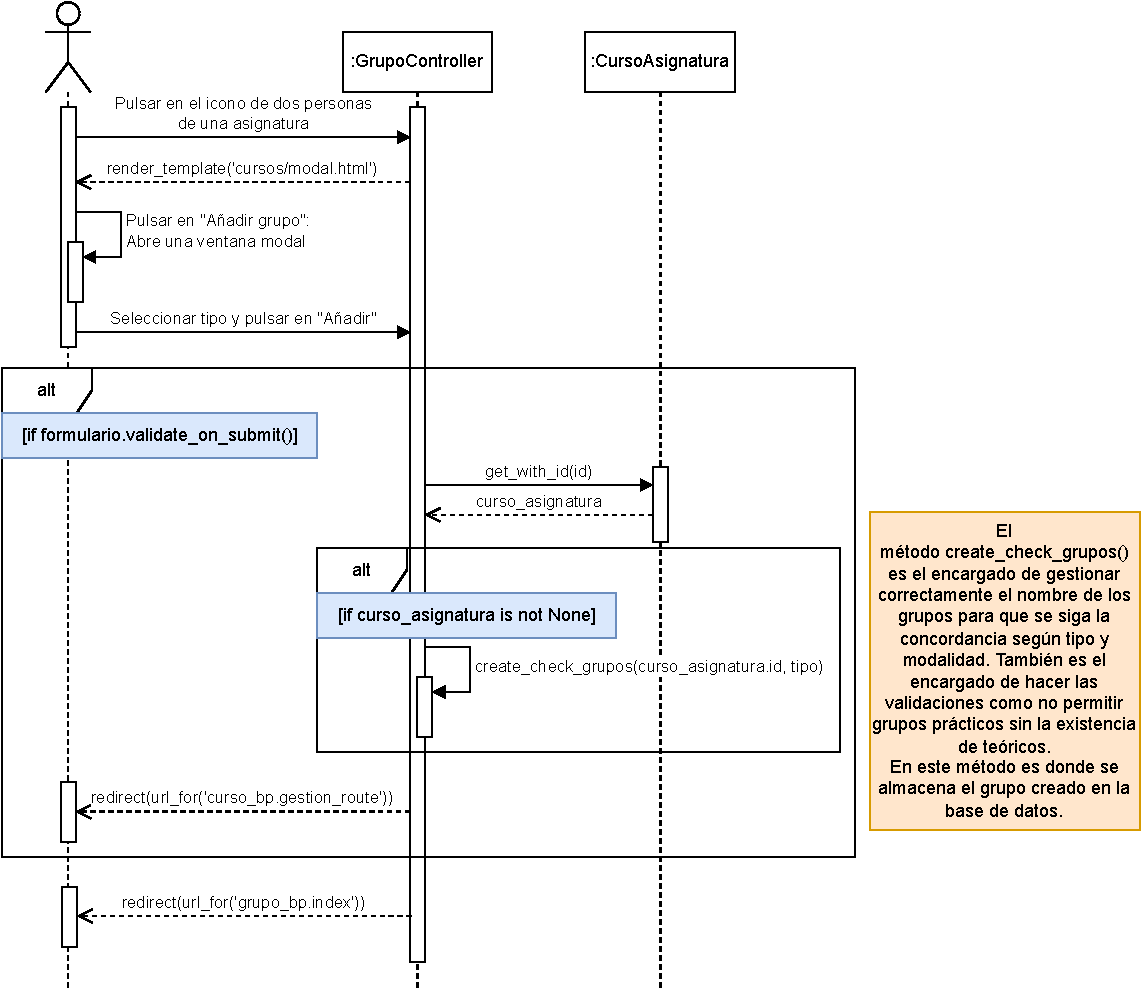
\includegraphics[width=\textwidth]{../img/Anexos/Diagramas secuencia/DS - crear grupo.pdf}
	\caption{Diagrama de secuencia de creación de grupos.}\label{DS-crearGrupo}
\end{figure}

\item \textbf{Asignación de horas de una plaza a un grupo}

El diagrama~\ref{DS-asignarHoras} representa la secuencia seguida para vincular una plaza a un grupo indicando el número de horas de docencia que va a impartir.

Se parte de que el usuario se encuentra en la ventana llamada <<Horas>> y que existe al menos un grupo y una plaza en la aplicación. 

El usuario pulsa sobre el icono del reloj de uno de los grupos de la lista que aparece en la pantalla. Esto abre una nueva ventana donde se pueden ver todos las plazas que cuentan con horas en ese grupo. El usuario pulsa en <<Añadir Plaza>>, lo que abre una ventana modal con un buscador mediante Ajax de la plaza y un campo para indicar las horas. El usuario selecciona una plaza e indica las horas y pulsa en <<Añadir>>.

De forma interna, el controlador de la plaza realiza una búsqueda de la plaza y grupo para asegurarse de que existen, con esta comprobación hecha se recogen las plazas del grupo. 
Si la plaza que se quiere asignar ya se encuentra en ese grupo no se permite, en caso contrario la plaza se vincula con las horas indicadas.

\begin{figure}
	\centering
	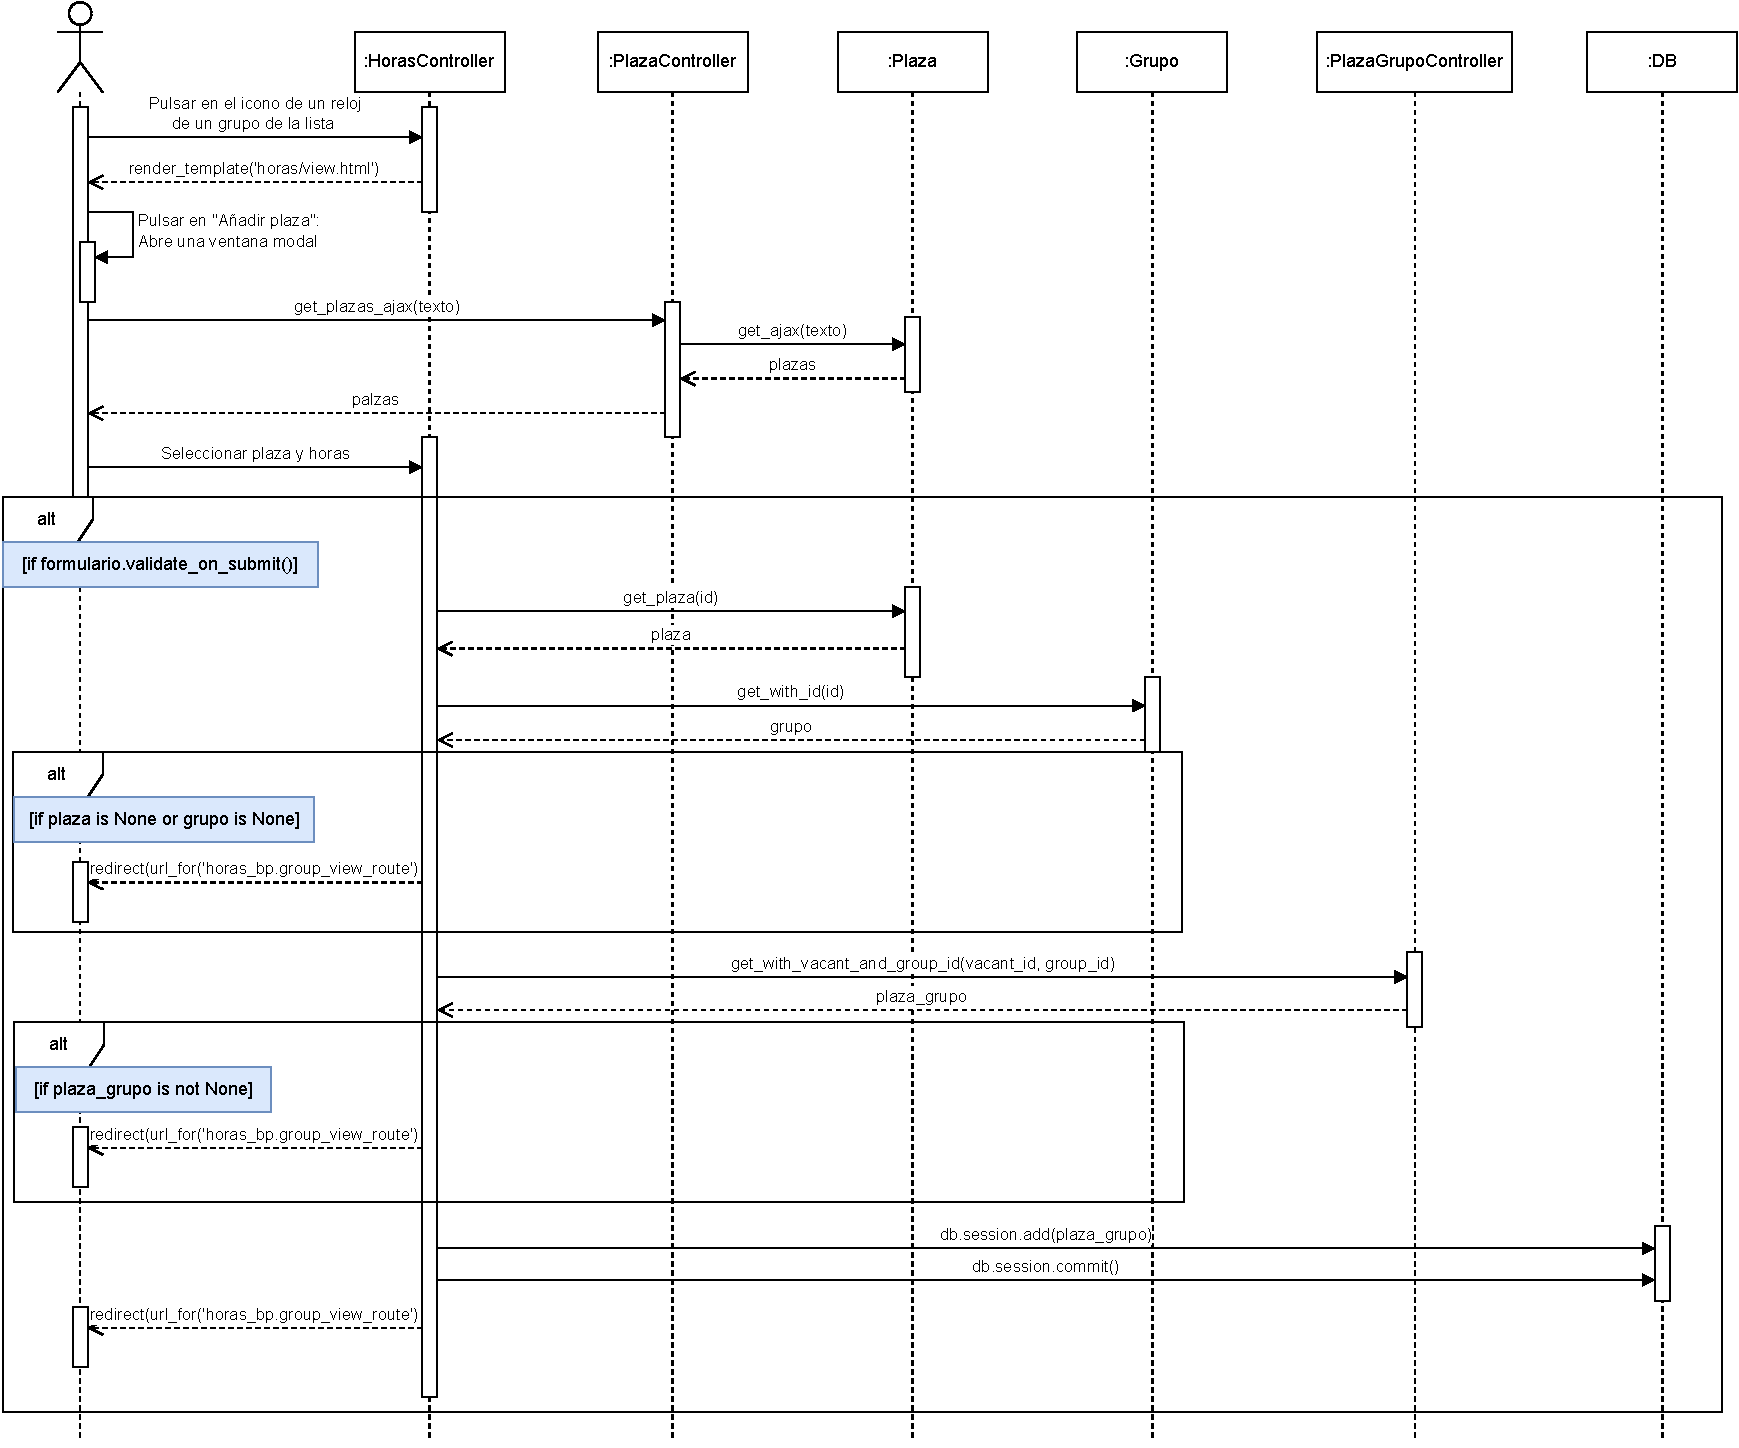
\includegraphics[width=\textwidth]{../img/Anexos/Diagramas secuencia/DS - asignar horas.pdf}
	\caption{Diagrama de secuencia de la asignación de horas de una plaza a un grupo.}\label{DS-asignarHoras}
\end{figure}

\end{itemize}


\section{Diseño arquitectónico}
El diseño arquitectónico define la estructura del \textit{software} creado respecto a la distribución de las clases y el patrón de diseño utilizado.

En este proyecto se ha seguido la arquitectura cliente-servidor bajo el patrón de diseño Modelo-vista-controlador (MVC).
Flask, que ha sido el \textit{framework} elegido para realizar el código de la aplicación, no obliga al uso de este patrón; sin embargo, se decidió utilizarlo se decidió utilizarlo debido a la organización que proporciona. 
Esto permite que el código quede separado de una forma fácil de entender, de modo que cualquier programador pueda identificar claramente la ubicación de cada elemento.

\begin{itemize}
\item \textbf{Modelo:}
Es el encargado del manejo de los datos de la aplicación.

\item \textbf{Vista:} 
Es la representación de los datos que ve el cliente de la web.
En este caso mediante código HTML bajo el uso del motor de plantillas Jinja2.

\item \textbf{Controlador:} 
Es la parte de la aplicación donde se encuentra la parte importante de la lógica.
Actúa de intermediario entre el cliente y los datos, recogiendo las peticiones de los clientes y haciendo las peticiones necesarias a los modelos para procesar la información requerida y devolver la respuesta al cliente a través de la vista.
\end{itemize}

En el diagrama~\ref{MVC} se representa el funcionamiento del MVC donde el usuario de la web interacciona, a través de la vista, con el controlador que se encarga de hacer peticiones y respuestas de datos con el modelo.
De esta forma el controlador es capaz de recuperar, modificar o eliminar los datos de un modelo.
Además, el controlador es el encargado de formar el código necesario para mostrar la vista que visualizará el usuario de la web.

\begin{figure}
	\centering
	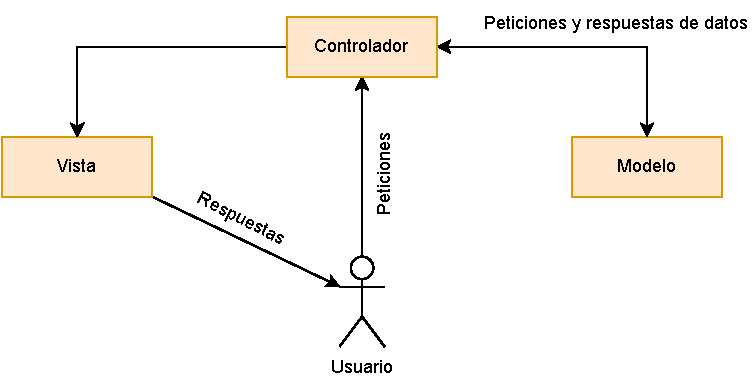
\includegraphics[width=\textwidth]{../img/Anexos/MVC.pdf}
	\caption{Modelo-Vista-Controlador}\label{MVC}
\end{figure}

También se ha incluido el diagrama de componentes~\ref{DiagramaComponentes} donde se puede ver de una forma más clara la estructura que tiene la aplicación web desarrollada.

\begin{figure}
	\centering
	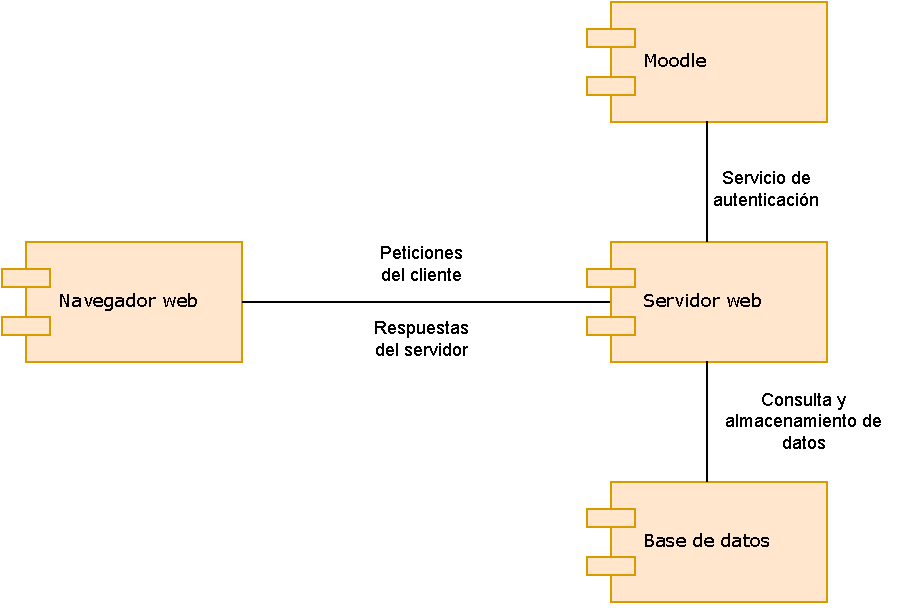
\includegraphics[width=\textwidth]{../img/Anexos/Diagrama componentes.pdf}
	\caption{Diagrama de componentes}\label{DiagramaComponentes}
\end{figure}





